% In this section, the layer is described in some detail in terms of its specific subsystems. Describe each of the layers and its subsystems in a separate chapter/major subsection of this document. The content of each subsystem description should be similar. Include in this section any special considerations and/or trade-offs considered for the approach you have chosen.

\subsection{Login Subsystem}
The Login Subsystem will be the first subsystem that users will interact with when first entering the application. This subsystem will allow users to login with their unique username or email, and their password. Once the credentials are confirmed to be correct, the system will redirect the user. 

\begin{figure}[h!]
	\centering
 	
\includegraphics[width=0.60\textwidth]{images/login}
 \caption{Login Subsystem}
\end{figure}

\subsubsection{Assumptions}
There will be the assumption that any user who attempts to login, will have already registered and received a unique username and set a password.

\subsubsection{Responsibilities}
The primary responsibility of the Login Subsystem will be to provide an interface for users to sign into the application. Upon receiving a users unique username or email and password, the Login Subsystem will relay these inputs to the Query Manager subsystem to be processed. The subsystem will then wait to receive confirmation. If the user entered credentials are incorrect, then the Login Subsystem will give an error message and prompt the user to re-enter their login information. If the credentials are correct, then the Login Subsystem will redirect the user to the home page.

\subsubsection{Subsystem Interfaces}
Each of the inputs and outputs for the subsystem are defined here.
\begin {table}[H]
\caption {Subsystem interfaces} 
\begin{center}
    \begin{tabular}{ | p{1cm} | p{4cm} | p{5cm} | p{5cm} |}
    \hline
    ID & Description & Inputs & Outputs \\ \hline
    \#1 & User Email or Unique Username and Password & \pbox{5cm}{Email or Username \\ Password} & \pbox{5cm}{Page Redirect or Error message}  \\ \hline
    \end{tabular}
\end{center}
\end{table}

\subsection{Register Subsystem}
The Registration Subsystem will allows new users to sign up and create their account with a unique email. Users should only need to use this subsystem once.

\begin{figure}[h!]
	\centering
 	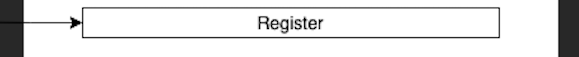
\includegraphics[width=0.60\textwidth]{images/register}
 \caption{Register Subsystem}
\end{figure}

\subsubsection{Assumptions}
There will be the assumption that all users who register have an email that they can access.

\subsubsection{Responsibilities}
The primary responsibility of the Register Subsystem is to provide an interface for users to sign up to use the application. Users will enter their email address, unique username, and password. Once the Register Subsystem receives these inputs, it will relay them to Query Management subsystem. If the user enters an email or username that is already being used, the Register Subsystem will display an error message and prompt the user for a new email or username. If the user's password does not match the certain requirements, then the system will display an error message and prompt the user to enter a new password. If the user gives all valid inputs, the Register Subsystem will give a confirmation and redirect the user to the login page.

\subsubsection{Subsystem Interfaces}
Each of the inputs and outputs for the subsystem are defined here.
\begin {table}[H]
\caption {Subsystem interfaces} 
\begin{center}
    \begin{tabular}{ | p{1cm} | p{6cm} | p{3cm} | p{3cm} |}
    \hline
    ID & Description & Inputs & Outputs \\ \hline
    \#1 & User Email, Unique Username, and Password & \pbox{3cm}{Email or Username \\ Password} & \pbox{3cm}{Page Redirect or Error message}  \\ \hline
    \end{tabular}
\end{center}
\end{table}

\subsection{Shopping List Subsystem}
The Shopping List Subsystem will provide an interface for users to search for their desired grocery item. This will also show users all the items that are currently on their shopping list.

\begin{figure}[h!]
	\centering
 	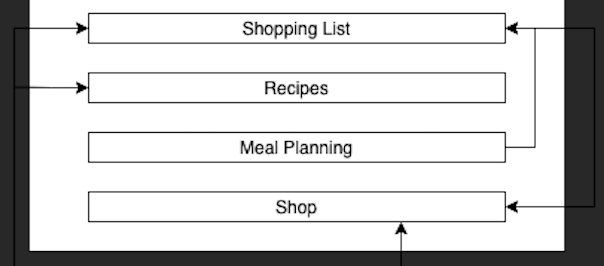
\includegraphics[width=0.60\textwidth]{images/shoppingList}
 \caption{Shopping List Subsystem}
\end{figure}

\subsubsection{Assumptions}
There are no assumptions for this subsystem.

\subsubsection{Responsibilities}
The Shopping List Subsystem will have two responsibilities. First it will communicate with the Query Manager subsystem to obtain the users current grocery list, it will then display this list for the user to see. The Shopping List Subsystem will also allow user to search for item to add to their list. 

Users will be able to type in the name of a desired grocery item. The system will send this input to the Query Manager to retrieve the results. This subsystem will then display all results. The user can the select the item they want. The Shopping List subsystem will send this selection to the Query Manager to be added to the users Shopping List.

Finally, if a user is ready to shop for all of their grocery items, they will select the option to shop and control will be transferred to the Shop Subsystem.

\subsubsection{Subsystem Interfaces}
Each of the inputs and outputs for the subsystem are defined here.
\begin {table}[H]
\caption {Subsystem interfaces} 
\begin{center}
    \begin{tabular}{ | p{1cm} | p{4cm} | p{5cm} | p{5cm} |}
    \hline
    ID & Description & Inputs & Outputs \\ \hline
    \#1 & Display Shopping List & \pbox{5cm}{-} & \pbox{5cm}{Shopping List from Query Manager}  \\ \hline
    \#2 & Grocery Item Search & \pbox{5cm}{Grocery Item from User} & \pbox{5cm}{User input to Query Manager}  \\ \hline
    \#3 & Search Results & \pbox{5cm}{Search Results from Query Manager} & \pbox{5cm}{Display Search Results to User}  \\ \hline
    \#4 & User Select Results & \pbox{5cm}{User Selected Item} & \pbox{5cm}{Selection to Query Manager}  \\ \hline
    \end{tabular}
\end{center}
\end{table}

\subsection{Recipes Subsystem}
The Recipes Subsystem will allow users to view recipes, add a recipe's ingredients to their shopping list, and add their own recipes.

\begin{figure}[h!]
	\centering
 	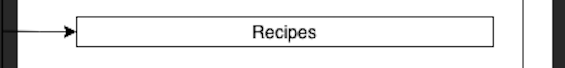
\includegraphics[width=0.60\textwidth]{images/recipes}
 \caption{Recipes Subsystem}
\end{figure}

\subsubsection{Assumptions}
User will be responsible for ensuring that recipes do not conflict with their dietary restrictions. It will also be assumed that users will not add dangerous recipes.

\subsubsection{Responsibilities}
The first responsibility of the Recipes Subsystem will be to provide an interface for users to view and search recipes. Upon entering the Recipes subsystem, users will be shown random recipes that were randomly pulled from the Query Manager. Users will then have the ability to search for recipes by using keywords or searching the name of known recipe. Upon receiving search text from the user, the system will relay that to the Query Manager to retrieve then display all results matching the search. 

After viewing the recipes, users will be able to select individual recipes. This will allow them to see all the ingredients and instructions. If the user likes the recipe, they will be able to add all the ingredients directly to their shopping list or meal plan.

The Recipes Subsystem will also enable user to share their own recipes. If a user decides to do this, users will first select all the ingredients and the amounts needed. After all ingredients are selected, the user will then be able to enter step-by-step instructions that describe how to create the recipe. Once this is complete, the system will send the user provided information to the Query Manager to be added to the recipe database.

\subsubsection{Subsystem Interfaces}
Each of the inputs and outputs for the subsystem are defined here.
\begin {table}[H]
\caption {Subsystem interfaces} 
\begin{center}
    \begin{tabular}{ | p{1cm} | p{4cm} | p{5cm} | p{5cm} |}
    \hline
    ID & Description & Inputs & Outputs \\ \hline
    \#1 & Recipe Search & \pbox{5cm}{User Search Text} & \pbox{5cm}{User Search Text to Query Manager}  \\ \hline
    \#2 & Recipe Search Results & \pbox{5cm}{Results of Search from Query Manager} & \pbox{5cm}{Search Results to User}  \\ \hline
    \#3 & Select Recipe to View & \pbox{5cm}{User Recipe Selection} & \pbox{5cm}{Recipe Selection to Query Manager}  \\ \hline
    \#4 & Display Recipe to View & \pbox{5cm}{Recipe Ingredients and Instruction from Query Manager} & \pbox{5cm}{Display Recipe Ingredients and Instruction}  \\ \hline
    \#5 & Add Recipe to Shopping List & \pbox{5cm}{User Choice to Add Recipe to Shopping List} & \pbox{5cm}{All Ingredients to Query Manager}  \\ \hline
    \#6 & Add Recipe to Meal Plan & \pbox{5cm}{User Choice to Add Recipe to Meal Plan} & \pbox{5cm}{Recipe ID to Query Manager}  \\ \hline
     \#7 & Add Own Recipe & \pbox{5cm}{All Ingredients and Instructions} & \pbox{5cm}{User Given Ingredients and Instructions to Query Manager}  \\ \hline
    \end{tabular}
\end{center}
\end{table}

\subsection{Meal Plan Subsystem}
The Meal Plan Subsystem will allow users to view and create a collection of recipes called Meal Plans. Users will be able to add recipes (via the Recipes Subsystem), delete recipes, and add all ingredients to the shopping list.

\begin{figure}[h!]
	\centering
 	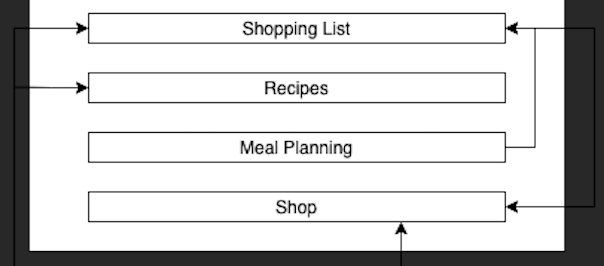
\includegraphics[width=0.60\textwidth]{images/shoppingList}
 \caption{Meal Plan Subsystem}
\end{figure}

\subsubsection{Assumptions}
Users will not be able to add ingredients that are not in a recipe to a Meal Plan.

\subsubsection{Responsibilities}
The Meal Plan Subsystem will allow users to create new Meal Plans that will be empty. Once a user chooses to do this, the Query Manager will be responsible for the creation of the Meal Plan in the database. A user will be able to add recipes to the their Meal Plan via the Recipes System. Once there is more than one recipe in a Meal Plan, the system will allow the user to view each Meal Plan and select ones to view individually. If a user selects a Meal Plan to view, the Meal Plan subsystem will retrieve all the its recipes through the Query Manager and display them to the user.

If a user decides they would like to use a Meal Plan, they will be able to add it to their shopping list. This will be done by adding getting all the ingredients from each recipe via the Query Manager and then adding them to the Shopping List.

\subsubsection{Subsystem Interfaces}
Each of the inputs and outputs for the subsystem are defined here.
\begin {table}[H]
\caption {Subsystem interfaces} 
\begin{center}
    \begin{tabular}{ | p{1cm} | p{4cm} | p{5cm} | p{5cm} |}
    \hline
    ID & Description & Inputs & Outputs \\ \hline
    \#1 & View Meal Plans & \pbox{5cm}{-} & \pbox{5cm}{All of the User's Meal Plans}  \\ \hline
    \#2 & Create Meal Plan & \pbox{5cm}{User Selection to Create a Meal Plan} & \pbox{5cm}{Creation Command to Query Manager}  \\ \hline
    \#3 & Select Single Meal Plan & \pbox{5cm}{User Meal Plan Selection} & \pbox{5cm}{Meal Plan Selection to Query Manager}  \\ \hline
    \#4 & View Single Meal Plan & \pbox{5cm}{Recipes in Meal Plan from Query Manager} & \pbox{5cm}{Display All Recipes to User}  \\ \hline
    \end{tabular}
\end{center}
\end{table}

\subsection{Shop Subsystem}
The Shop Subsystem will act as an interface to present users with the optimal grocery trip. 

\begin{figure}[h!]
	\centering
 	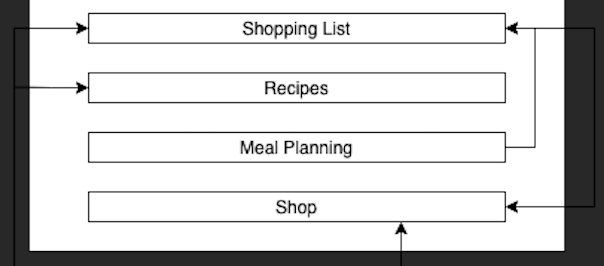
\includegraphics[width=0.60\textwidth]{images/shoppingList}
 \caption{Shop Subsystem}
\end{figure}

\subsubsection{Assumptions}
There are no assumptions for this subsystem.

\subsubsection{Responsibilities}
The system will access the Shop Subsystem via the Shopping List Subsystem when a user decides they are ready to shop for the grocery items on their list. Once the subsystem receives the grocery items from the list, it will send that information to the Shopping Manager Subsystem along with the user defined preferences. All calculation will be done on the Server Layer. Once the Shop Subsystem receives the results, it will display the stores the user should visit, the items they will get at each stores, the sequence the stores should be visited, and a link to a map application to navigate their route.

\subsubsection{Subsystem Interfaces}
Each of the inputs and outputs for the subsystem are defined here.
\begin {table}[H]
\caption {Subsystem interfaces} 
\begin{center}
    \begin{tabular}{ | p{1cm} | p{4cm} | p{5cm} | p{5cm} |}
    \hline
    ID & Description & Inputs & Outputs \\ \hline
    \#1 & Initiate Shopping & \pbox{5cm}{Shopping List Items \\ User Preferences} & \pbox{5cm}{Shopping List Items and User Preferences to the Shopping Manager}  \\ \hline
    \#2 & Display Results & \pbox{5cm}{Optimal Shopping Trip From Shopping Manager} & \pbox{5cm}{Display Optimal Shopping Trip to User}  \\ \hline
    \end{tabular}
\end{center}
\end{table}




